\section{Core matching and alternating force response}
The two independently selectable core controls use projection recoloring
and the raw D2Q9 spectrum explicitly specified by Liu et al.
\cite{liu2015}. The standard row order is density, energy, energy square,
$j_x,q_x,j_y,q_y,p_{xx},p_{xy}$ (with corresponding coordinate reversal
in the internal arrays). Rates are
$(1,1.63,1.14,1,1.92,1,1.92,1/\tau,1/\tau)$.
Production operator output, pure force integration and actual outgoing
recoloring populations are checked independently. Conserved moment rates
one are compatible with net force: $j^{eq}-j=F/2$ and the Guo prefactor
supplies the other half. Their rate value does not by itself damp a
post-stream state that is already an equilibrium.

For standard D2Q9 coordinate/diagonal weights $a,b$, projection has axial
segregation $B_p=a+2b=A$. Its reflected wall has $B_{p,w}=a+b=A_w$.
Thus the stationary ratio is already the same, while the transient wall
clock remains $5/6$ of the bulk clock. A cosine-derived multiplier must
not be applied again. With
$\beta_p=\beta_c(a+\sqrt{2}b)/(a+2b)$, the entire axial bulk recurrence
matches the recovered cosine formulation. At $\beta_c=0.7$ the six
calibrations, covering both spectra and three recoloring strengths,
give matched profiles within $\CoreMatchedProfileError$.
Independent projection equilibria verify the local bounce-back fixed
point. Conservative wall transfer additionally preserves the matched
complete transient at every early step, including odd times.

Second recoloring tensors are scalar in both formulations, so this beta
match also matches their leading second moment. The unscaled cosine
tensor has $T_{xx}=0.300789642$, $T_{xxxx}=T_{xx}$ and
$T_{xxyy}=0.0785674201$. The projection tensor has
$T_{xx}=T_{xxxx}=1/3$ and $T_{xxyy}=1/9$.
This fourth-moment difference can affect multidimensional transport;
it is not an attribution of every measured wall discrepancy.
The 45-degree normal widths are 4.719891 (cosine), 4.330870
(projection at beta 0.7), and 4.716003 (matched projection).
Normal sample spacing is $1/\sqrt2$ instead of the axial spacing one,
and linear-crossing interpolation also contributes to these comparisons.

An early width diagnostic mistakenly selected the positive/negative
0.9 crossings of different periodic interfaces, giving width 64.
Raw simulation input did not contain that width. The preserved run
receipts retain the original metadata, and the collector explicitly
replaces it in a copy with independently calibrated same-interface width.
Pressure and all numerical populations are unchanged; circle-fit
diagnostics are recomputed with the correct width.

For an alternating component, incoming raw momentum is $P_t-G_t/2$.
Local collision adds $G_t$, so outgoing momentum is $P_t+G_t/2$.
Each nonzero-axis streaming link changes alternating spatial sign;
wall reflection reverses that component at the same site. For the even
periodic axis or a complete reflecting wall-normal axis,
$P_{t+1}=-P_t+(G_{t+1}-G_t)/2$ follows without a fitted coefficient.
The production force audit reads the same color as the native outgoing
state; physical velocity comes from incoming-state VTI fields.
Mean projections use fluid-node count and density-weighted velocity.
Eight adjacent states give residual below $5.1\times10^{-19}$.

\begin{figure}[htbp]\centering
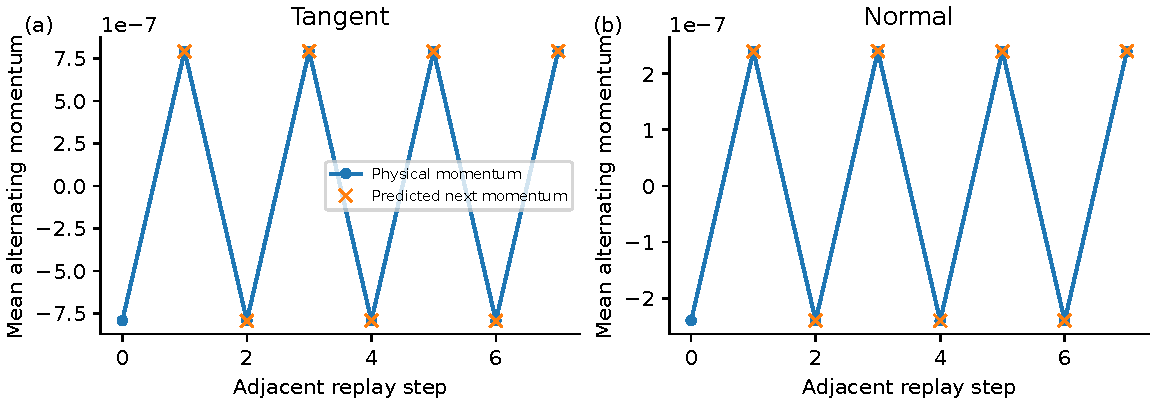
\includegraphics[width=.98\linewidth]{figures/parity-force.pdf}
\caption{Actual alternating physical momentum and the independently
predicted next value in the held 60-degree ghost/phase-transfer control.
The force/streaming identity concerns a known lattice mode, not a new
hydrodynamic eigenvalue or a velocity filter.\AIPlotDisclosure}
\end{figure}

After setting sigma to zero for 2048 steps, the maximum raw speed is
$8.00\times10^{-7}$ and the adjacent-average diagnostic is
$2.28\times10^{-10}$. Alternating tangential/normal momentum amplitudes
remain approximately $7.92\times10^{-7}$ and $1.10\times10^{-7}$.
An odd periodic length removes the even-periodic tangent identity but
retains the wall-normal mode and changes the geometry slightly. An
exact one-cell translation preserves every field. The inherited fixed
bulk-pressure windows do not translate, producing a $4.739\times10^{-6}$
relative sampled difference; that is a sampling effect, not loss of
translation covariance. SRT and both MRT controls preserve exact
checkerboard equilibria and avoid false steady termination.

Eight bulk droplet runs at R12/R24, followed by four-duration R24 holds,
retain input sigma 0.005. At R12, relative Laplace discrepancies are
approximately 1.388--1.404\%; held R24 discrepancies are
0.303--0.306\%. Maximum unfiltered speed decreases with projection;
pressure calibration is not adjusted to match the slit.
Separate pure force-driven channels check
$C=4(\tau-1/2)(1/s_q-1/2)/3-1/4$ at three widths and three tau values.
The relative mean flux shift is $12C/(2H^2+1)$.

\section{Pressure collars, budgets and finite-time drift}
The extension retains Zou--He reconstruction in a pure force-free collar.
Its guard is evaluated on outgoing populations before stream and incoming
densities after boundary reconstruction. Both PB planes must cover the
outer fluid faces, prescribe consistent phase/density and point inward
on one common axis. Complete walls must be parallel to that axis.
The PB plane and two interior strips have other-phase fraction below
$10^{-9}$; the first interior strip's actual color-gradient norm must be
below $10^{-9}$. PB capillary arrays stay zero. The interface therefore
cannot be allowed to cross a pressure boundary in this experiment.

Relative-phase transfers vanish on all wall faces touching PB. Kinetic
inflow uses outgoing PB populations directed into interior VD/GV;
outflow uses outgoing interior populations directed to PB. Solid-link
reflection returns mass and is not counted as external flux.
Compensated cumulative sums and independently read field sums test
each component. Accounting restarts at the loaded outgoing time;
MPI/restart comparisons retain bitwise fields and populations, but
accumulated budget baselines naturally differ.

Twenty-four pure pressure channels cover H8/H16/H32, tau1/tau1.55,
both spectra, both phases and both drive signs. The central midpoint
profile uses the measured density gradient without fitting velocity.
Its maximum relative discrepancy is $1.92\times10^{-5}$; the endpoint
gradient assumption itself differs by up to approximately 0.450\%.

Closed donor total populations are preserved in the single-front map:
for $x<H$, use donor $2H$ and combine into phase0; for $H\le x<3H$,
use donor $x+H$; for $x\ge3H$, use donor 0 and combine into phase1.
The target outgoing clock is one. Every donor/target checkpoint hash,
phase collapse and clock change is recorded. No force, beta or velocity
is calibrated to a desired dynamic outcome.

At H16/H32, cosine/legacy MRT and matched projection with either spectrum
share 60-degree walls and equal tau1. The broad three-pressure sequence
is held to four initial durations. A separate pair has prespecified
width $0.0005p_Y$ centered on the independently measured closed pressure;
both drift signs are verified at both durations. Estimated zero ratios
come from a three-point linear response and are not thermodynamic
thresholds. Centerline and first-fluid-row crossings remain distinct
from volume-equivalent position and from a physical wall contact line.

\begin{table}[htbp]\centering\small
\caption{Flat-slit closed/dynamic pressure consistency and measured front mobility. The pressure pair has width $0.0005\,p_Y$ and is tested at both durations; the linear zero estimate uses the three broad pressure values. Mobility includes contact-line/interface effects and is not assigned to a universal numerical error.}
\begin{tabular}{llrrrr}\toprule
Recoloring & MRT & $H$ & Closed offset (\%) & Dynamic offset (\%) & Mobility shift (\%) \\ \midrule
Cosine & Legacy & 16 & +1.841 & +1.847 & -11.43 \\
Cosine & Legacy & 32 & +1.186 & +1.190 & -17.73 \\
Projection & Legacy & 16 & +0.517 & +0.519 & -11.26 \\
Projection & Legacy & 32 & -0.336 & -0.334 & -17.57 \\
Projection & Published & 16 & +0.551 & +0.552 & -11.59 \\
Projection & Published & 32 & -0.341 & -0.340 & -17.82 \\
\bottomrule\end{tabular}\end{table}


The raw fields retain capillary circulation. A separate zero-sigma
experiment, using the same donor and reservoir pressure, diagnoses
decoupled total-fluid transport; it is not a capillary prediction.
Moving-contact-line dissipation and regularization have established
theory \cite{huh1971}. The present slope differences do not distinguish
a numerical contact-line mobility from all physical viscous contributions.
Slip calibration, rate convergence, fixed physical interface thickness,
wall orientation, higher resolution and an actual throat geometry remain
separate physical tests.
